\documentclass[a4paper, 12pt]{article}%тип документа



%отступы
\usepackage[left=1cm,right=1cm,top=1cm,bottom=2cm,bindingoffset=0cm]{geometry}

%%% Работа с русским языком
\usepackage{graphicx}
\usepackage{cmap}                           % поиск в PDF
\usepackage{mathtext} 			 	       % русские буквы в формулах
\usepackage[T2A]{fontenc}               % кодировка
\usepackage[utf8]{inputenc}              % кодировка исходного текста
\usepackage[english,russian]{babel} 
\usepackage{float}

\usepackage[export]{adjustbox} % локализация и переносы

\usepackage{subfig}% http://ctan.org/pkg/subfig
\usepackage{booktabs}

\usepackage{wrapfig}


%Матеша
\usepackage{amsmath,amsfonts,amssymb,amsthm,mathtools} % AMS
\usepackage{icomma} % "Умная" запятая

%\mathtoolsset{showonlyrefs=true} % Показывать номера только у тех формул, на которые есть \eqref{} в тексте.

%% Шрифты
\usepackage{euscript}	 % Шрифт Евклид
\usepackage{mathrsfs} % Красивый матшрифт

%% Свои команды
\DeclareMathOperator{\sgn}{\mathop{sgn}}

%% Перенос знаков в формулах (по Львовскому)
\newcommand*{\hm}[1]{#1\nobreak\discretionary{}
	{\hbox{$\mathsurround=0pt #1$}}{}}




\author{Гаврилин Илья Дмитриевич \\
	Б01-101}
\title{\textbf{Работа 2.2.3 \\ 
		Определение теплопроводности газов	\\при атмосферном давлении}}

\begin{document}
	\maketitle
	\section{Аннотация}
	В работе получен коэффициент теплопроводности воздуха ($k \left[ \dfrac{\text{Вт}}{\text{м} \cdot \text{К}} \right]$) при атмосферном давлении в зависимости от температуры. Определен коэффициент $\beta$ в формуле: $k(T)\sim T^{\beta}$. Также, оценен тепловой коэффициент сопротивления $\alpha$ для молибдена. Расчитаны погрешности полученных величин.
	\section{Теоритические сведения}
	\textit{Теплопроводность} — это процесс передачи тепловой энергии от нагретых частей системы к холодным за счёт хаотического движения частиц среды (молекул, атомов и т.п.). В газах теплопроводность осуществляется за счёт  непосредственной передачи кинетической энергии от быстрых молекул к медленным при их столкновениях. Перенос тепла описывается законом Фурье, утверждающим, что плотность потока энергии $\overline{q} = -k \nabla T$, где $k \left[ \dfrac{\text{Вт}}{\text{м} \cdot \text{К}} \right]$ - \textit{коэффициент теплопроводности}.
	
	Молекулярно-кинетическая теория дает следующую оценку для коэффициента теплопроводности газов: 
	
	\begin{equation} 
		k \sim \lambda \overline{\nu} \cdot n c_V, \overline{\nu} = \sqrt{\frac{8kT}{\pi m}}
	\end{equation}
	С помощью некоторых преобразований мы получаем, что: 
	\begin{equation} 
		Q = \dfrac{2 \pi L}{\ln \dfrac{r_0}{r_1}} k  \cdot \Delta T 
	\end{equation}
	\subsection{Экспериментальная установка}
		Установка состоит из термостата, нагревающего воздух вокруг исследуемой проволоки, электрической схемы коммутации и замера тока и напряжения на исследуемой проволоке (Рис. 2). Исследуемая проволока находится в металлическом цилиндре, вокруг которого проходит рубашка водяного нагревателя (Рис. 1).
		\begin{figure}[H]
			\begin{center}
				\begin{minipage}[h]{0.4\linewidth}
					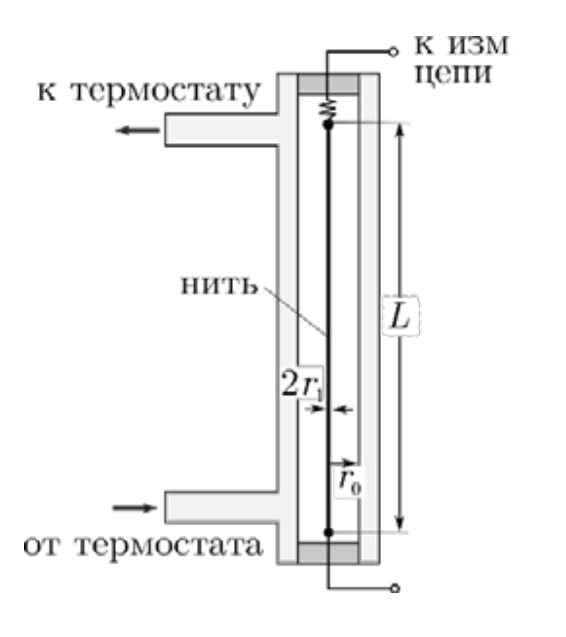
\includegraphics[width=1\linewidth]{scheme}
					\caption{Устройство колбы с нитью} %% подпись к рисунку
				\end{minipage}
				\hfill
				\begin{minipage}[h]{0.4\linewidth}
					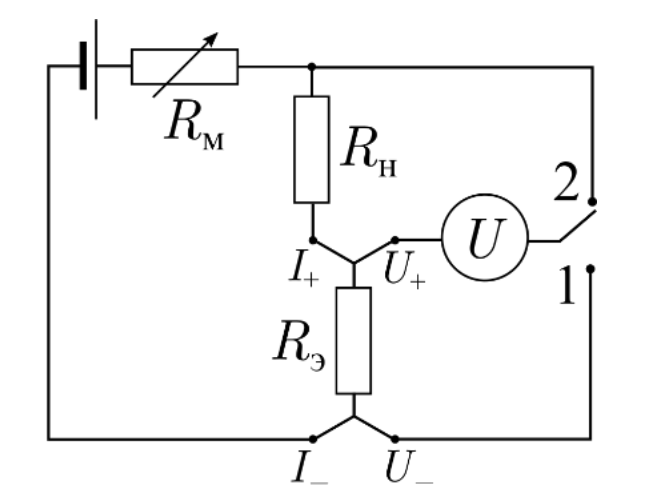
\includegraphics[width=1\linewidth]{electric}
					\caption{Схема измерения тока и напряжения на проволоке}
					
					
				\end{minipage}
				
			\end{center}
		\end{figure}
	Параметры указанные на рисунках установки:\\ 
	\begin{center}
		$L=347~мм; D_{0} = 2r_{0} = 10\pm0.1~мм;D_{1} = 2r_{1} = 0.05\pm 0.005~мм; R_{э}=10\pm0.001~Ом$
	\end{center}
	\section{Ход работы}
	Подберем такие значения сопротивления магазина сопротивлений($R_{м}$), что мощность нагрева будет равномерно расти в соответствии с коэффициентом $\alpha$.
	\begin{table}[H]
		\centering
		\begin{tabular}{|c|c|c|c|c|c|c|c|c|c|c|c|}
			\hline
			$\alpha$ & 1 & 0.9  & 0.8 & 0.7 & 0.6 & 0.5 & 0.4  & 0.3  & 0.2  & 0.1  & 0.01 \\ \hline
			$R_{м}, Ом$     & 0 & 1.48 & 1.6 & 4.3 & 6.4 & 9.1 & 12.6 & 18.2 & 27.2 & 47.6 & 198  \\ \hline
		\end{tabular}
		\caption{Подбор сопротивлений для установки параметров.}
	\end{table}
	Проведем эксперимент для замера теплопроводности воздуха при комнатной температуре\\ (T = 295 K). Путем вычислений получим выделяемую на проволоке мощность и ее сопротивление. Из этих данных построим график R(Q), аппроксимирую его прямой получим значение $\frac{dR}{dQ}$, а также сопротивление проволоки при этой температуре, то есть при нулевой мощности($R_{0}$).
	\begin{table}[H]
		\centering
		\begin{tabular}{|c|c|c|c|c|}
			\hline
			$\alpha$ & $V_{н}, ~ В$ & $V_{э}, ~ В$ & R, Ом & Q Дж \\ \hline
			0.01  & 0.265   & 0.182     & 14.560  & 0.005      \\ \hline
			0.1   & 0.823   & 0.560     & 14.696  & 0.046      \\ \hline
			0.2   & 1.154   & 0.777     & 14.852  & 0.090      \\ \hline
			0.3   & 1.403   & 0.936     & 14.989  & 0.131      \\ \hline
			0.4   & 1.620   & 1.071     & 15.126  & 0.174      \\ \hline
			0.5   & 1.793   & 1.175     & 15.260  & 0.211      \\ \hline
			0.6   & 1.953   & 1.270     & 15.378  & 0.248      \\ \hline
			0.7   & 2.098   & 1.354     & 15.495  & 0.284      \\ \hline
			0.8   & 2.319   & 1.478     & 15.690  & 0.343      \\ \hline
			0.9   & 2.355   & 1.498     & 15.721  & 0.353      \\ \hline
		\end{tabular}
		\caption{Мощность и сопротивление нити при комнатной температуре (T = 295 K).}
	\end{table}
	\begin{figure}[H]
		\centering
		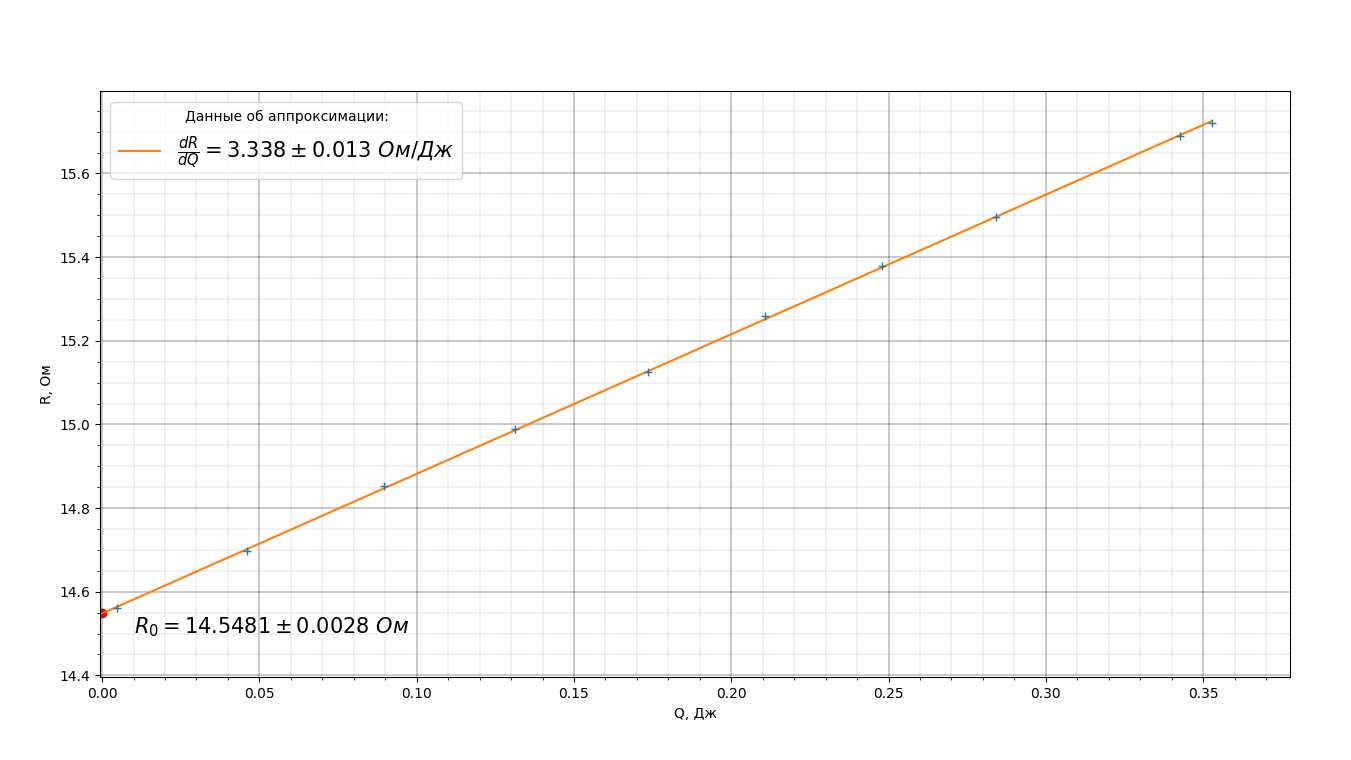
\includegraphics[width=0.8\linewidth]{22_grad}
		\caption{Зависимость сопротивления проволоки от выделяемой мощности(T = 295 K).}
		\label{fig:22grad}
	\end{figure}
	Аналогичные рассуждения проведем для 4 оставшихся значений температур, составим таблицу и построим графики.
	\begin{table}[H]
		\centering
		\begin{tabular}{|ccccc|ccccc|}
			\hline
			\multicolumn{5}{|c|}{T = 303 K}                                                                                                            & \multicolumn{5}{c|}{T = 313 K}                                                                                                            \\ \hline
			\multicolumn{1}{|c|}{$\alpha$} & \multicolumn{1}{c|}{$V_{н}, ~ В$} & \multicolumn{1}{c|}{$V_{э}, ~ В$} & \multicolumn{1}{c|}{R, Ом} & Q, Дж & \multicolumn{1}{c|}{$\alpha$} & \multicolumn{1}{c|}{$V_{н}, ~ В$} & \multicolumn{1}{c|}{$V_{э}, ~ В$} & \multicolumn{1}{c|}{R, Ом} & Q, Дж \\ \hline
			\multicolumn{1}{|c|}{0.01}  & \multicolumn{1}{c|}{0.272}   & \multicolumn{1}{c|}{0.182}     & \multicolumn{1}{c|}{14.945}  & 0.005      & \multicolumn{1}{c|}{0.01}  & \multicolumn{1}{c|}{0.279}   & \multicolumn{1}{c|}{0.182}     & \multicolumn{1}{c|}{15.330}  & 0.005      \\ \hline
			\multicolumn{1}{|c|}{0.1}   & \multicolumn{1}{c|}{0.839}   & \multicolumn{1}{c|}{0.557}     & \multicolumn{1}{c|}{15.063}  & 0.047      & \multicolumn{1}{c|}{0.1}   & \multicolumn{1}{c|}{0.859}   & \multicolumn{1}{c|}{0.554}     & \multicolumn{1}{c|}{15.505}  & 0.048      \\ \hline
			\multicolumn{1}{|c|}{0.2}   & \multicolumn{1}{c|}{1.174}   & \multicolumn{1}{c|}{0.772}     & \multicolumn{1}{c|}{15.207}  & 0.091      & \multicolumn{1}{c|}{0.2}   & \multicolumn{1}{c|}{1.198}   & \multicolumn{1}{c|}{0.766}     & \multicolumn{1}{c|}{15.640}  & 0.092      \\ \hline
			\multicolumn{1}{|c|}{0.3}   & \multicolumn{1}{c|}{1.425}   & \multicolumn{1}{c|}{0.929}     & \multicolumn{1}{c|}{15.339}  & 0.132      & \multicolumn{1}{c|}{0.3}   & \multicolumn{1}{c|}{1.451}   & \multicolumn{1}{c|}{0.919}     & \multicolumn{1}{c|}{15.789}  & 0.133      \\ \hline
			\multicolumn{1}{|c|}{0.4}   & \multicolumn{1}{c|}{1.642}   & \multicolumn{1}{c|}{1.061}     & \multicolumn{1}{c|}{15.476}  & 0.174      & \multicolumn{1}{c|}{0.4}   & \multicolumn{1}{c|}{1.670}   & \multicolumn{1}{c|}{1.049}     & \multicolumn{1}{c|}{15.920}  & 0.175      \\ \hline
			\multicolumn{1}{|c|}{0.5}   & \multicolumn{1}{c|}{1.816}   & \multicolumn{1}{c|}{1.164}     & \multicolumn{1}{c|}{15.601}  & 0.211      & \multicolumn{1}{c|}{0.5}   & \multicolumn{1}{c|}{1.843}   & \multicolumn{1}{c|}{1.149}     & \multicolumn{1}{c|}{16.040}  & 0.212      \\ \hline
			\multicolumn{1}{|c|}{0.6}   & \multicolumn{1}{c|}{1.976}   & \multicolumn{1}{c|}{1.257}     & \multicolumn{1}{c|}{15.720}  & 0.248      & \multicolumn{1}{c|}{0.6}   & \multicolumn{1}{c|}{2.004}   & \multicolumn{1}{c|}{1.240}     & \multicolumn{1}{c|}{16.161}  & 0.248      \\ \hline
			\multicolumn{1}{|c|}{0.7}   & \multicolumn{1}{c|}{2.121}   & \multicolumn{1}{c|}{1.339}     & \multicolumn{1}{c|}{15.840}  & 0.284      & \multicolumn{1}{c|}{0.7}   & \multicolumn{1}{c|}{2.148}   & \multicolumn{1}{c|}{1.321}     & \multicolumn{1}{c|}{16.260}  & 0.284      \\ \hline
			\multicolumn{1}{|c|}{0.8}   & \multicolumn{1}{c|}{2.340}   & \multicolumn{1}{c|}{1.460}     & \multicolumn{1}{c|}{16.027}  & 0.342      & \multicolumn{1}{c|}{0.8}   & \multicolumn{1}{c|}{2.365}   & \multicolumn{1}{c|}{1.438}     & \multicolumn{1}{c|}{16.446}  & 0.340      \\ \hline
			\multicolumn{1}{|c|}{0.9}   & \multicolumn{1}{c|}{2.376}   & \multicolumn{1}{c|}{1.474}     & \multicolumn{1}{c|}{16.119}  & 0.350      & \multicolumn{1}{c|}{0.9}   & \multicolumn{1}{c|}{2.401}   & \multicolumn{1}{c|}{1.457}     & \multicolumn{1}{c|}{16.479}  & 0.350      \\ \hline
			\multicolumn{5}{|c|}{T = 323 K}                                                                                                            & \multicolumn{5}{c|}{T = 333 K}                                                                                                            \\ \hline
			\multicolumn{1}{|c|}{$\alpha$} & \multicolumn{1}{c|}{$V_{н}, ~ В$} & \multicolumn{1}{c|}{$V_{э}, ~ В$} & \multicolumn{1}{c|}{R, Ом} & Q, Дж & \multicolumn{1}{c|}{$\alpha$} & \multicolumn{1}{c|}{$V_{н}, ~ В$} & \multicolumn{1}{c|}{$V_{э}, ~ В$} & \multicolumn{1}{c|}{R, Ом} & Q, Дж \\ \hline
			\multicolumn{1}{|c|}{0.01}  & \multicolumn{1}{c|}{0.287}   & \multicolumn{1}{c|}{0.181}     & \multicolumn{1}{c|}{15.856}  & 0.005      & \multicolumn{1}{c|}{0.01}  & \multicolumn{1}{c|}{0.295}   & \multicolumn{1}{c|}{0.181}     & \multicolumn{1}{c|}{16.298}  & 0.005      \\ \hline
			\multicolumn{1}{|c|}{0.1}   & \multicolumn{1}{c|}{0.879}   & \multicolumn{1}{c|}{0.550}     & \multicolumn{1}{c|}{15.982}  & 0.048      & \multicolumn{1}{c|}{0.1}   & \multicolumn{1}{c|}{0.900}   & \multicolumn{1}{c|}{0.547}     & \multicolumn{1}{c|}{16.453}  & 0.049      \\ \hline
			\multicolumn{1}{|c|}{0.2}   & \multicolumn{1}{c|}{1.222}   & \multicolumn{1}{c|}{0.759}     & \multicolumn{1}{c|}{16.100}  & 0.093      & \multicolumn{1}{c|}{0.2}   & \multicolumn{1}{c|}{1.247}   & \multicolumn{1}{c|}{0.752}     & \multicolumn{1}{c|}{16.582}  & 0.094      \\ \hline
			\multicolumn{1}{|c|}{0.3}   & \multicolumn{1}{c|}{1.477}   & \multicolumn{1}{c|}{0.909}     & \multicolumn{1}{c|}{16.249}  & 0.134      & \multicolumn{1}{c|}{0.3}   & \multicolumn{1}{c|}{1.504}   & \multicolumn{1}{c|}{0.900}     & \multicolumn{1}{c|}{16.711}  & 0.135      \\ \hline
			\multicolumn{1}{|c|}{0.4}   & \multicolumn{1}{c|}{1.697}   & \multicolumn{1}{c|}{1.037}     & \multicolumn{1}{c|}{16.365}  & 0.176      & \multicolumn{1}{c|}{0.4}   & \multicolumn{1}{c|}{1.724}   & \multicolumn{1}{c|}{1.025}     & \multicolumn{1}{c|}{16.820}  & 0.177      \\ \hline
			\multicolumn{1}{|c|}{0.5}   & \multicolumn{1}{c|}{1.871}   & \multicolumn{1}{c|}{1.138}     & \multicolumn{1}{c|}{16.441}  & 0.213      & \multicolumn{1}{c|}{0.5}   & \multicolumn{1}{c|}{1.898}   & \multicolumn{1}{c|}{1.121}     & \multicolumn{1}{c|}{16.931}  & 0.213      \\ \hline
			\multicolumn{1}{|c|}{0.6}   & \multicolumn{1}{c|}{2.031}   & \multicolumn{1}{c|}{1.224}     & \multicolumn{1}{c|}{16.593}  & 0.249      & \multicolumn{1}{c|}{0.6}   & \multicolumn{1}{c|}{2.058}   & \multicolumn{1}{c|}{1.207}     & \multicolumn{1}{c|}{17.051}  & 0.248      \\ \hline
			\multicolumn{1}{|c|}{0.7}   & \multicolumn{1}{c|}{2.175}   & \multicolumn{1}{c|}{1.302}     & \multicolumn{1}{c|}{16.705}  & 0.283      & \multicolumn{1}{c|}{0.7}   & \multicolumn{1}{c|}{2.201}   & \multicolumn{1}{c|}{1.283}     & \multicolumn{1}{c|}{17.155}  & 0.282      \\ \hline
			\multicolumn{1}{|c|}{0.8}   & \multicolumn{1}{c|}{2.391}   & \multicolumn{1}{c|}{1.416}     & \multicolumn{1}{c|}{16.886}  & 0.339      & \multicolumn{1}{c|}{0.8}   & \multicolumn{1}{c|}{2.417}   & \multicolumn{1}{c|}{1.395}     & \multicolumn{1}{c|}{17.326}  & 0.337      \\ \hline
			\multicolumn{1}{|c|}{0.9}   & \multicolumn{1}{c|}{2.426}   & \multicolumn{1}{c|}{1.435}     & \multicolumn{1}{c|}{16.906}  & 0.348      & \multicolumn{1}{c|}{0.9}   & \multicolumn{1}{c|}{2.452}   & \multicolumn{1}{c|}{1.413}     & \multicolumn{1}{c|}{17.353}  & 0.346      \\ \hline
		\end{tabular}
			\caption{Мощность и сопротивление нити при температурах, отличных от комнатной.}
	\end{table}
	\begin{figure}[H]
		\begin{center}
			\begin{minipage}[h]{0.48\linewidth}
				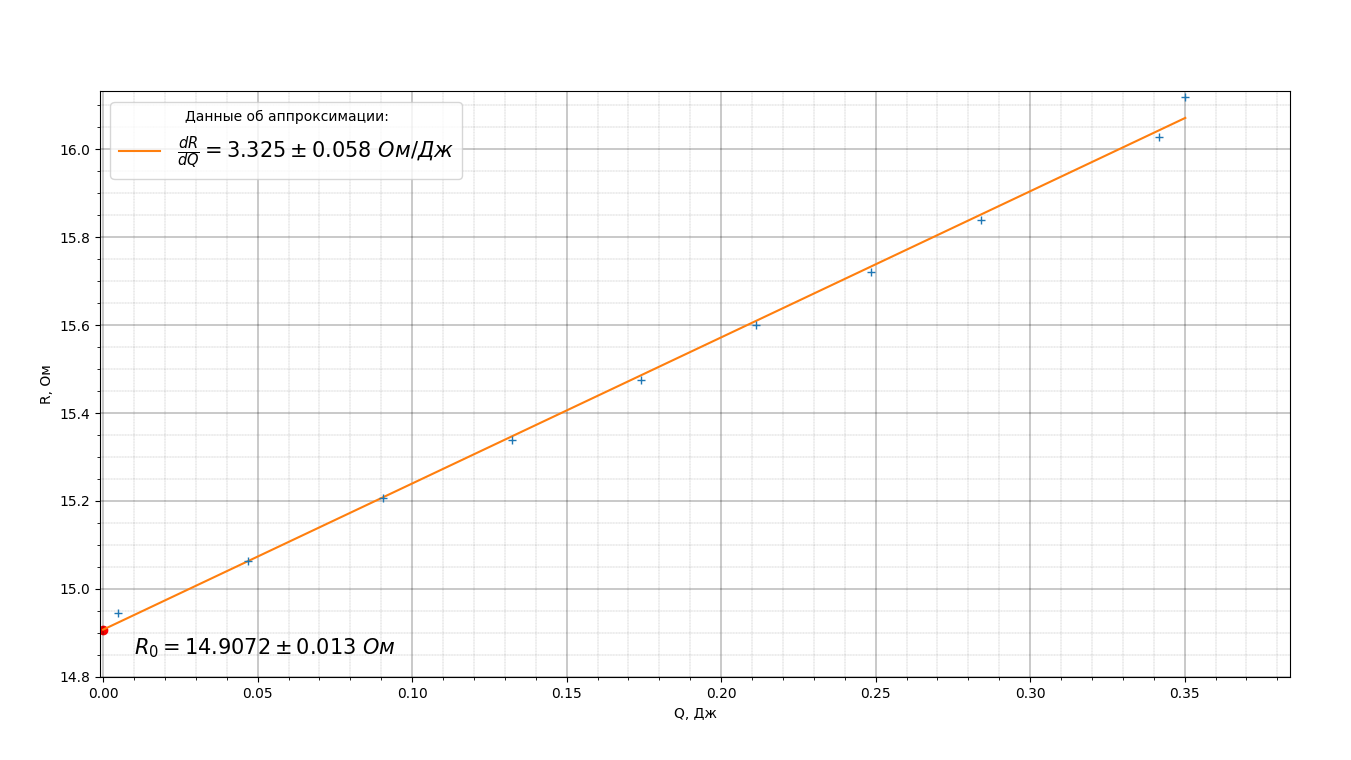
\includegraphics[width=1\linewidth]{30_grad}
				\caption{T = 303 K} 
			\end{minipage}
			\hfill
			\begin{minipage}[h]{0.48\linewidth}
				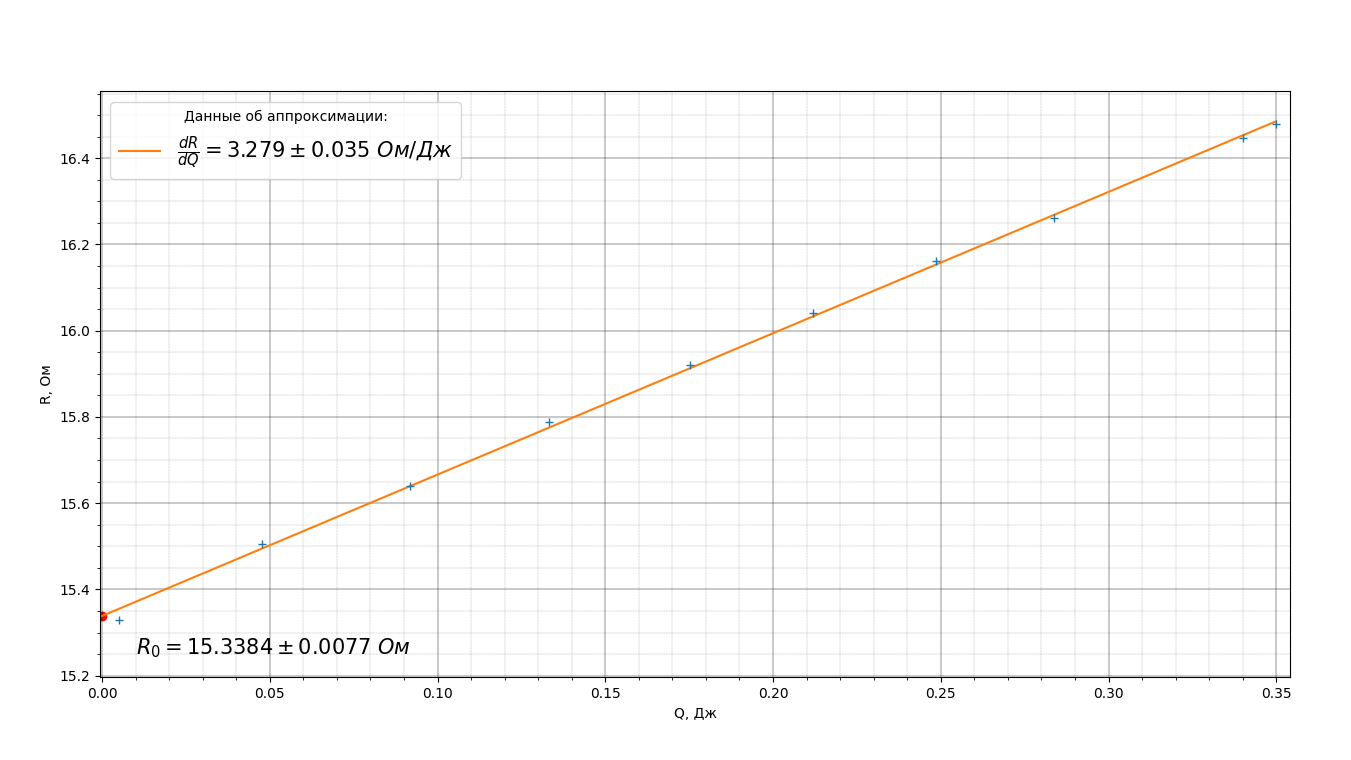
\includegraphics[width=1\linewidth]{40_grad}
				\caption{T = 313 K}
				
				
			\end{minipage}
		\end{center}
		\begin{center}
			\begin{minipage}[h]{0.48\linewidth}
				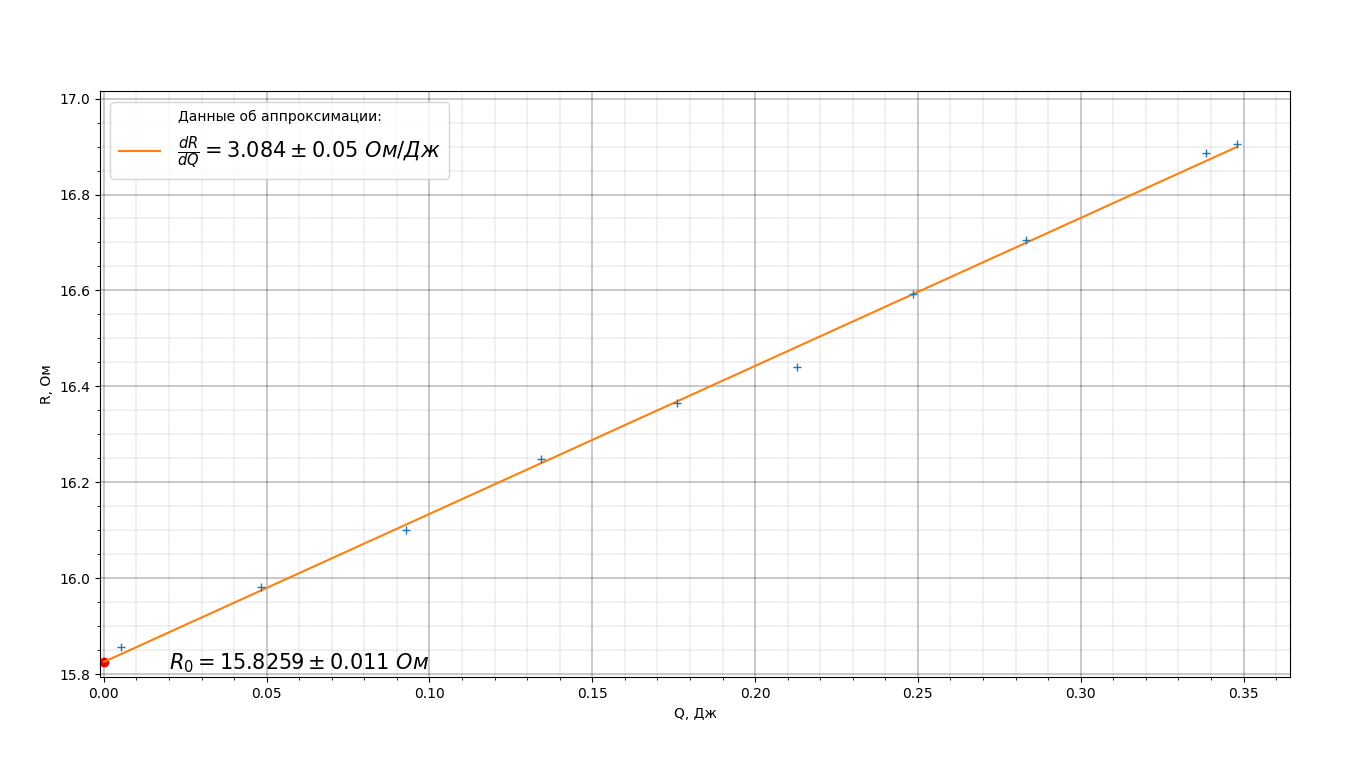
\includegraphics[width=1\linewidth]{50_grad}
				\caption{T = 323 K} %% подпись к рисунку
			\end{minipage}
			\hfill
			\begin{minipage}[h]{0.48\linewidth}
				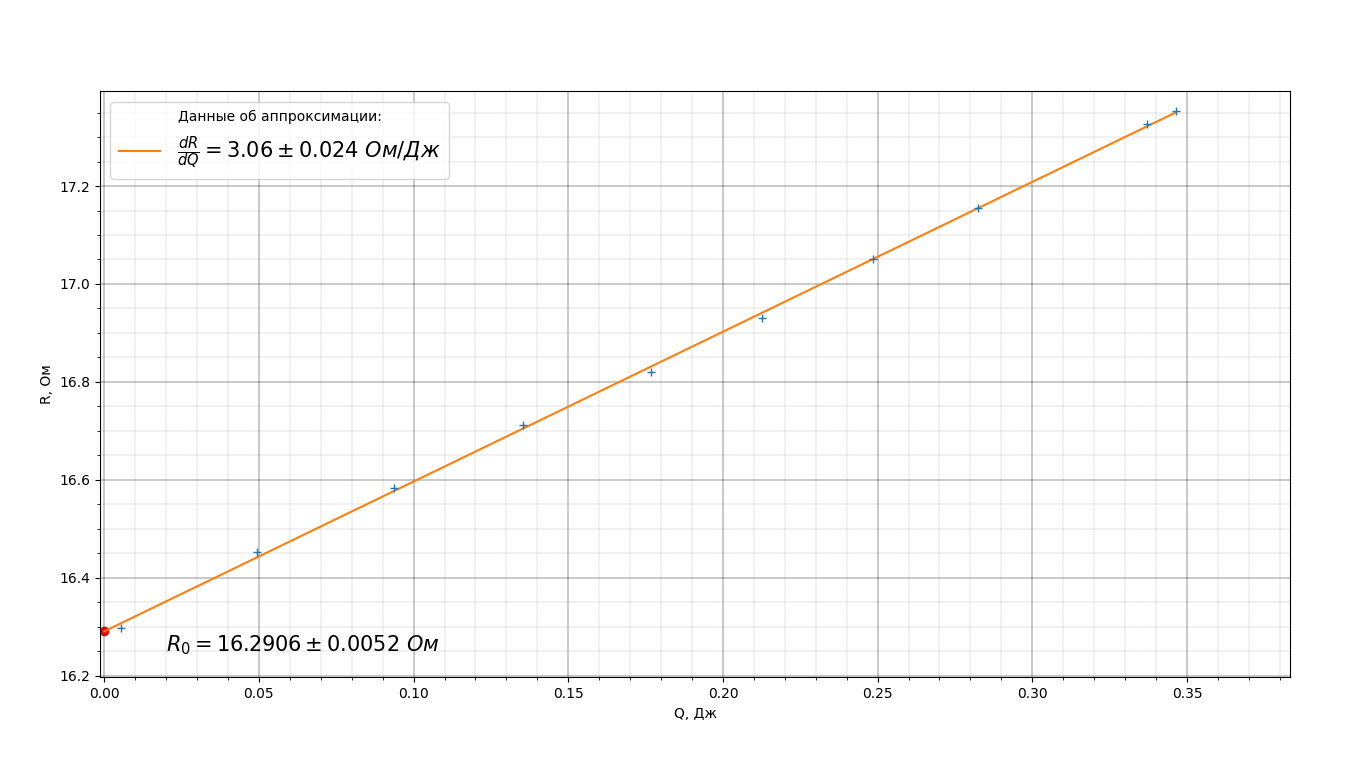
\includegraphics[width=1\linewidth]{60_grad}
				\caption{T = 333 K}
			\end{minipage}
		\end{center}
	\caption*{Зависимости сопротивлений проволоки от выделяемой мощности при различных температурах}
	\end{figure}
	Построим таблицу полученных из аппроксимаций значений, сразу вычислим $\frac{dQ}{d\Delta T}$(см. Рис. 8).
	\begin{table}[H]
		\centering
		\begin{tabular}{|c|c|c|c|c|l|l|}
			\hline
		T, K & $R_{0}, Ом$   & $\sigma(R), Ом$ & $\frac{dR}{dQ}, Ом/Дж$ & $\sigma(\frac{dR}{dQ}), Ом/Дж$ & \multicolumn{1}{c|}{$\frac{dQ}{d\Delta T}~ Дж/К$} & \multicolumn{1}{c|}{k}\\ \hline
			295  & 14.5481 & 0.003  & 3.338 & 0.013       & 0.01372                     & $0.0333 \pm 0.002$                 \\ \hline
			303  & 14.907 & 0.013  & 3.325 & 0.058       & 0.01377                     & $0.0335 \pm 0.002$                \\ \hline
			313  & 15.338 & 0.007  & 3.279 & 0.035       & 0.01397                     & $0.0339 \pm 0.002$                 \\ \hline
			323  & 15.826 & 0.011  & 3.084 & 0.050       & 0.01485                     & $0.0361 \pm 0.003$                 \\ \hline
			333  & 16.291 & 0.005  & 3.062 & 0.024       & 0.01496                     & $0.0364 \pm 0.003$               \\ \hline
		\end{tabular}
	\caption{Данные, полученные из аппроксимаций графиков R(Q)}
	\end{table}
	По полученным данным $R_{0}$ построим график зависимости $R(T)$, по нему определим тепловой коэффициент зависимости сопротивления и $\frac{dR}{dT}$.
	Для температурного коэффициента зависимости сопротивления:
	\begin{equation}
		\alpha = \frac{1}{R_{273}}\frac{dR}{dT} = 0.0034 ~\frac{1}{C};
		~\alpha_{табл} = 0.0046 ~\frac{1}{C};~ \epsilon = 26 \%
	\end{equation}
	Построим в логарифмическом масштабе график: $ln~k/k_{0}(ln~T/T_{0})$, по нему определим коэффициент $\beta$ в формуле $k \sim T^{\beta}$(см. Рис. 9).

	 \begin{figure}[H]
	 	\begin{center}
	 		\begin{minipage}[h]{0.48\linewidth}
	 			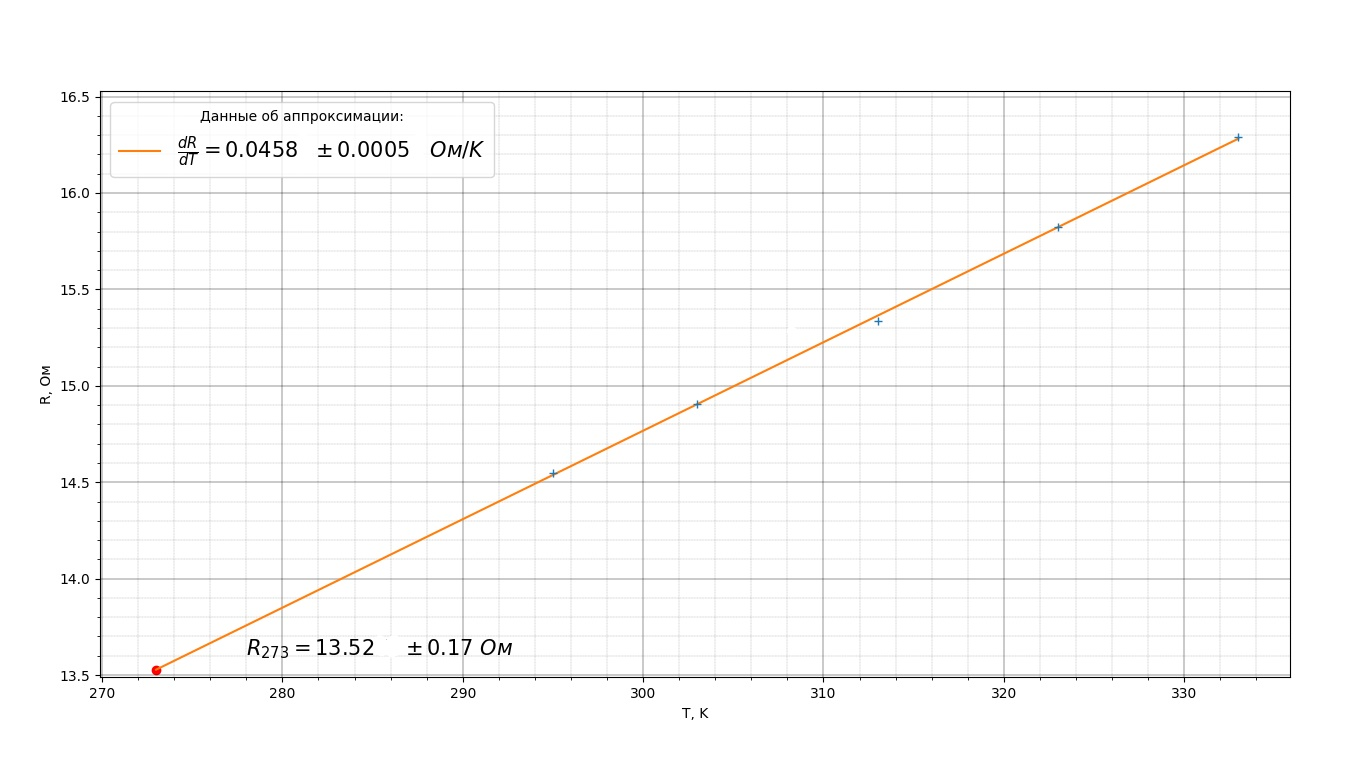
\includegraphics[width=1\linewidth]{InkedR_T_LI}
	 			\caption{Зависимость сопротивления проволоки от температуры}
	 		\end{minipage}
	 		\hfill
	 		\begin{minipage}[h]{0.48\linewidth}
	 			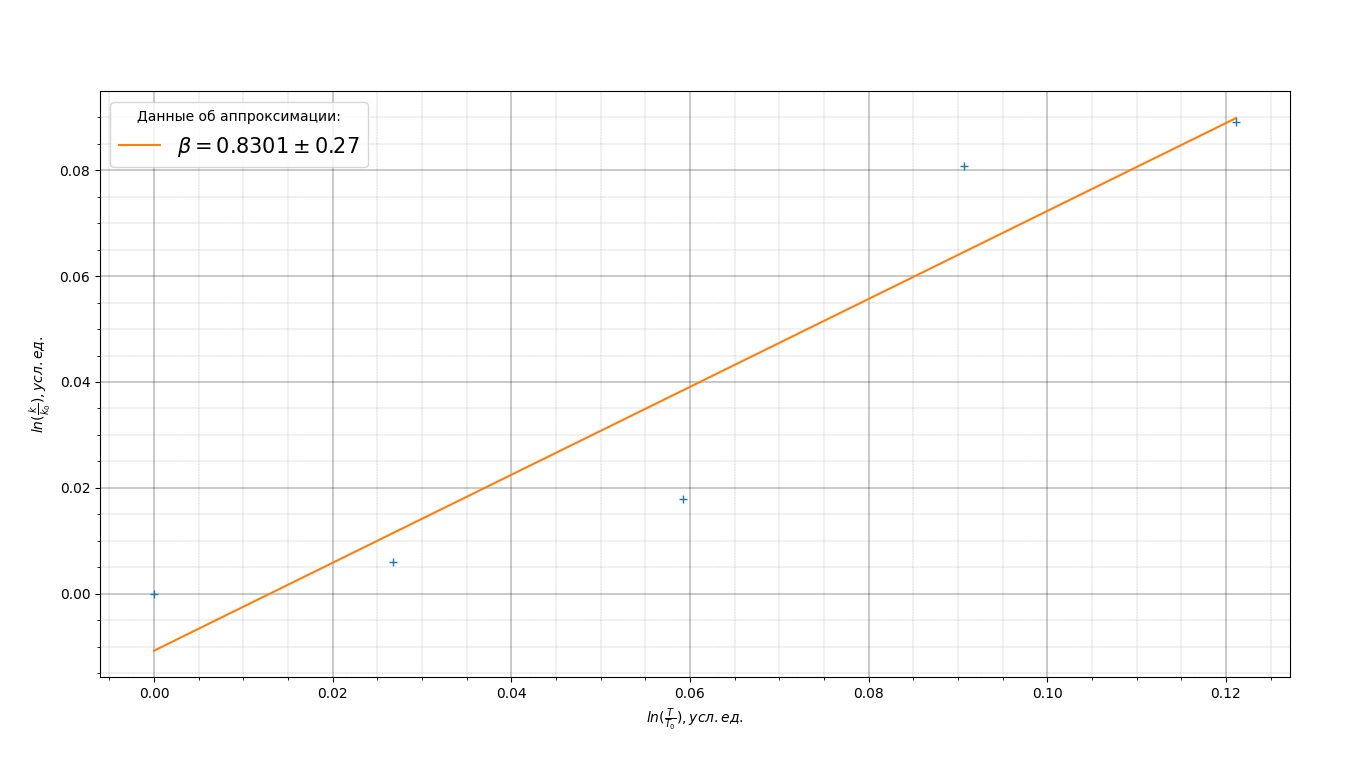
\includegraphics[width=1\linewidth]{beta}
	 			\caption{Зависимость $ln~k/k_{0}(ln~T/T_{0})$}
	 			
	 			
	 		\end{minipage}
	 	\end{center}
 	\end{figure}
	 \section{Выводы}
	 1. Нашли тепловой коэффициент зависимости сопротивления для молибдена $\alpha = 0.0034 \frac{1}{C}$, погрешность его определения составила $26\%$.\\
	 2. Определили степень в зависимости коэффициента теплопроводности воздуха от температуры $\beta = 0.83\pm 0.27$, хотя из теоретических предположений $\beta = 0.5$.\\
	 3. Оценили значения теплопроводности воздуха при нормальном давлении для разных температур.\\
	 \begin{table}[H]
	 	\centering
	 	\begin{tabular}{|c|c|c|c|}
	 		\hline
	 		T, K & $k_{эксп}$ & $k_{табл}$ & $\epsilon$ \\ \hline
	 		295  & 0.033   & 0.026     & 0.291   \\ \hline
	 		303  & 0.034   & 0.026     & 0.279   \\ \hline
	 		313  & 0.034   & 0.027     & 0.260   \\ \hline
	 		323  & 0.036   & 0.028     & 0.303   \\ \hline
	 		333  & 0.036   & 0.029     & 0.277   \\ \hline
	 	\end{tabular}
 		\caption{Сравнение полученного и эталонного коэффициента теплопроводности}
	 \end{table}
	 4. Проанализировав данные модно заметить что погрешность определения теплопроводности не зависит от температуры, а также нет больших различий в погрешностях, что косвенно доказывает отсутствие ошибок в измерении конкретной серии значений, также об отсутствии ошибок можно судить по тому, что экспериментальные точки и зависимость сопротивления от температуры прекрасно ложатся на прямую. \textbf{Подводя итог, хотелось бы выразить предположение что ошибка может появится ввиду:}\\
	 4.1 Плохого электрического контакта в рубильнике и соединительных проводах(особенно между проволокой и проводами вольтметра).\\
	 4.2 Слабого теплоотвода трубы и недостижения достаточно большой разницы температур.\\
	 4.3 Появления конвекционных потоков внутри трубки с проволокой(или же напротив неоднородности температуры воздуха относительно всей длины проволоки).\\
	4.4 Того, что представленные методы дают большую погрешность при отсутствии прямого снятия показаний тока и напряжения непосредственно с измеряемой проволоки.\\
\end{document}